\chapter{Background}
\label{ch:background}
This chapter offers some summaries of and references to background material and knowledge that is useful to have when studying the work done in the next chapters. 

\section{The Lua Programming Language}
\label{sec:lua_language}

The Lua programming language is a dynamic, multi-paradigm scripting language developed at the \gls{puc-rio}. It is implemented and maintained by a team of only three people: professors Roberto Ierusalimschy and Waldemar Celes of \gls{puc-rio}, and researcher Luiz Henrique de Figueiredo of \gls{impa}. Lua is designed as an embeddable extension language, and considered to be one of the leading scripting languages in game development~\cite{inproceedings:the_evolution_of_lua}. A likely reason for Lua's popularity is that the designers set some goals for the language's design and implementation that have been respected from the beginning: Lua should be embeddable, simple, efficient, portable and lightweight~\cite{article:the_implementation_of_lua}.

\noindent
This section only aims to give a general impression of the Lua programming language.  Below, some of the key properties of Lua are listed, to give an overview of the programming language's capabilities.
\begin{itemize}
	\item Lua is dynamically typed and interpreted, similar to languages like Python and Ruby.
	\item Lua uses only a single kind of data structure, which is an associative array (or simply \emph{table} in Lua). Additionally, all values in Lua are \emph{first-class} values, meaning they can be passed between functions and scopes, and stored in variables~\cite[ch. 2.2]{manual:lua_reference_manual}.
	\item Lua has simple and minimalist syntax~\cite[ch. 9]{manual:lua_reference_manual}. However, this does not necessarily make Lua itself simplistic, because of the meta-mechanisms that provide implicit support for many additional paradigms~\cite[ch. 2.8]{manual:lua_reference_manual}.
	\item Lua code is compiled to bytecode, and run in the register-based Lua \gls{vm}. This register-based \gls{vm} is part of what makes Lua efficient~\cite{article:the_implementation_of_lua}.
	\item The Lua \gls{vm} is written in \gls{clean-c}, and additionally offers quick and easy integration with C libraries. This is primarily what makes Lua portable.
	\item The Lua core only contains a few standard libraries. The reason for this is to avoid bloating, and decreasing the cost of embedding Lua. Extensions may be added as user libraries~\cite{article:the_implementation_of_lua}. Not including a lot of standard libraries goes a long way in keeping the memory footprint of Lua low.
	\item Lua supports collaborative (non-preemptive) multitasking in the form of coroutines~\cite[ch. 2.6]{manual:lua_reference_manual}. While this is not considered ``real'' multitasking (everything is done sequentially even on an application-level), this concept can be used to implement multitasking behavior by explicit context switching. For example, we can design a program to continuously run a working loop while frequently checking for input, without having to worry about interrupts. 
	\item Included in Lua's tiny core is an incremental mark-and-sweep garbage collector, which has a few advantages (no extra overhead, simple handling of cycles) and disadvantages (possible execution pause during collection) compared to other common types of garbage collectors. Automatic memory handling greatly reduces the difficulty of using the programming language for less experienced programmers.
	\item Lua is distributed under the very liberal MIT license, stating that Lua is open source and may be used for any purpose at no cost~\cite{website:lua_license}.
\end{itemize}

\noindent
While Lua is designed as an extension scripting language mainly for C applications, it is still possible to execute standalone Lua programs through the Lua interpreter~\cite[ch. 7]{manual:lua_reference_manual}.

\noindent
In addition to games, Lua is also used in various other types of applications and contexts. Some of these are database management, \glspl{ide}, image processing, web and browsers, multimedia, text editors and even operating systems~\cite{website:where_lua_is_used}. Among some of the more famous non-game applications we find Adobe Photoshop Lightroom, GIMP and Wireshark.

\noindent
Some work has also been done towards using Lua in embedded environments. This is discussed further in Sect.~\ref{sec:lua_in_embedded}. Additionally, Sect.~\ref{sec:lua_and_state_machines} discusses some of Lua's characteristics when considered in a state machine systems context.

\section{State Machine Systems}
\label{sec:state_machine_system}
A \gls{fsm} is a concept for modeling the behavior of a real or abstract program in a clear and structured way. An \gls{fsm} has a number of possible \emph{states}, of which it is always in one, and a number of \emph{transitions} describing conditions for changing from one state to another, typically in the form of an input signal. Additionally, these transitions may describe \emph{operations} that should be performed as part of the transition. There are many different ways to model \glspl{fsm}, and two common examples are UML statechart diagrams and SDL state diagrams.

\noindent
Figure~\ref{fig:fsm_example} shows an example of a simple \gls{fsm} for a code-keypad controlling a door, modeled in SDL. This simple program defines two states, \emph{idle} and \emph{waiting}, as well as some signals describing the possible transitions between them.

\begin{figure}[htp]
	\centering
	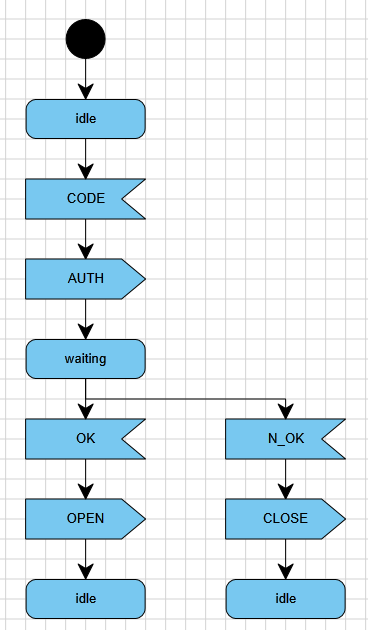
\includegraphics[scale=0.50]{stm_example}
	\caption[SDL finite-state machine example]{An example finite-state machine for accessing a door, modeled in SDL.}
	\label{fig:fsm_example}
\end{figure}

\noindent
\glspl{fsm} may be used for describing a vast amount of different types of systems, but used in conjunction with concepts like \glspl{msc} and collaborations, they are particularly effective for describing complex systems that display concurrent and distributed behavior. Models like these allow for \emph{conceptual abstraction} and \emph{separation of concerns}, allowing developers to reduce a complex system into simpler collaborating components~\cite{article:itut_methodologies}.

\noindent
When a system has been modeled through the use of these concepts, developers begin the process of translating the specifications to working code. This allows the system specification to be independent of the actual implementation, with the added bonus that the models serve as documentation (diagrams are generally easier to read and understand than numerous lines of code). Building on these concepts, it is possible to develop tools both for model verification and code generation~\cite{article:compositional_arctis}. Various tools already exist for these purposes, and some of these are discussed in Sect.~\ref{sec:existing_frameworks_state_machine}.

\noindent
Another way of working with \glspl{fsm} is to provide a \emph{runtime system} for an arbitrary set of different \gls{fsm} implementations. We then create a framework to handle most of the underlying implementation concerns, like message passing, timers, signal handling and the like, and provide a general interface to this framework for arbitrary \gls{fsm} implementations. Given a working, robust and efficient runtime system, it becomes simple for developers to create applications, as they only need to specify and implement the behavior of the application in terms of \glspl{fsm} and operations. Going even further, one can provide modeling tools with automatic code generation, reducing the developer's workload even more. This additionally reduces the room for errors and makes applications easier to maintain and extend.

\noindent
There are many more good reasons for and ways to use state machine modeling and other related semantics for designing software.\footnote{\cite{article:itut_methodologies},~\cite{chapter:structural_modeling_uml},~\cite{conference:system_analysis_modeling},~\cite{phd:frank}} This project focuses on the implementation of a runtime system with an interface for running arbitrary state machines, as discussed in the previous paragraph, in the Lua programming language.

\section{Embedded Systems and M2M}
\label{sec:embedded_m2m}
Embedded systems are computer devices designed for specific purposes, working as a part of a larger system. These devices usually have both specialized hardware and software, tailored to the task they are meant to perform. There are vast numbers of practical applications for embedded systems, but a few examples of such devices are Internet routers, mp3-players, thermostats and dishwashers.

\noindent
One of the most important aspects when designing embedded devices is to keep the costs low (they are often produced in great numbers), meaning most embedded devices have far sparser capabilities than for example home computers. The core of an embedded device is often a microcontroller, and different types offer different capabilities. Some of the smallest use 8-bit CPUs, have less than 1KB of available program memory and only a few registers for working memory, and are only a few millimeters wide.\footnote{\url{http://www.atmel.com/devices/ATTINY4.aspx}} On the other hand, the largest microcontrollers have up to 100KB ram, 512KB of program memory and use generally faster up to 32-bit CPUs.\footnote{\url{http://arduino.cc/en/Main/arduinoBoardDue}} Going even further, we find \glspl{soc} like the popular Raspberry Pi,\footnote{\url{http://www.raspberrypi.org/faqs}} capable of running desktop operating systems and with support for numerous peripherals.

\noindent
Embedded devices are often associated with the concept \emph{\gls{iot}},\footnote{\url{http://www.internet-of-things.eu/}} which describes the development towards increased amounts of \gls{m2m}-applications and devices that are a part of our daily lives, such as home automation and smart grids.\footnote{\url{http://smartgrids.no/}} The available types and applications of such devices is steadily increasing, and research is being done in many fields related to \gls{iot}.

\noindent
With the increasing use of embedded systems and smart devices, and the vast range of possible uses, it may become attractive for users to be able to create their own applications. In the current market, there are few \emph{do-it-yourself}-solutions for regular users, and even for (less experienced) programmers, programming embedded devices can be a significant challenge. Often one has to dive into low-level programming languages and deal with issues that require intimate knowledge of the hardware devices. In order to enable less experienced programmers and possibly regular users to create their own applications, the development must be taken to a higher abstraction level. One possible way of doing this is to use the concept of state machines, as described in Sect.~\ref{sec:state_machine_system}. If developers only need to specify their application on a state machine -level, it significantly reduces the amount of knowledge and experience required to build applications, and this even provides advantages for the more experienced.